\documentclass[class=report,crop=false, 12pt]{standalone}
\usepackage[screen,nosolutions]{../scratch}

\begin{document}

\titre[S]{Entrée/Sortie}
%===============================

\insertvideo{delXHz33zC8}{Entrée/Sortie -- Activité 1}

\insertvideo{p9Ms6wE9X5o}{Entrée/Sortie -- Activité 2}

\insertvideo{TDo_UAN-vZ0}{Entrée/Sortie -- Activité 3}

\bigskip
\bigskip


\begin{activite}
Programme Scratch afin qu'il réagisse en fonction des commandes suivantes :
\begin{itemize}
  \item les touches de flèches font monter, descendre Scratch ou le font aller vers la gauche ou la droite,
  \item la touche \mot{m} fait jouer un son,
  \item la touche \mot{c} passe au costume suivant,
  \item la touche \mot{espace} change la couleur du stylo de $10$,
  \item la touche \mot{f} efface tout l'écran.
\end{itemize}
\textbf{Bonus 1.} La touche \mot{r} relève le stylo, la touche \mot{s} place le stylo en position d'écriture.

\textbf{Bonus 2.} Trouve d'autres actions à contrôler avec des touches et trace de beaux dessins !

\begin{center}
  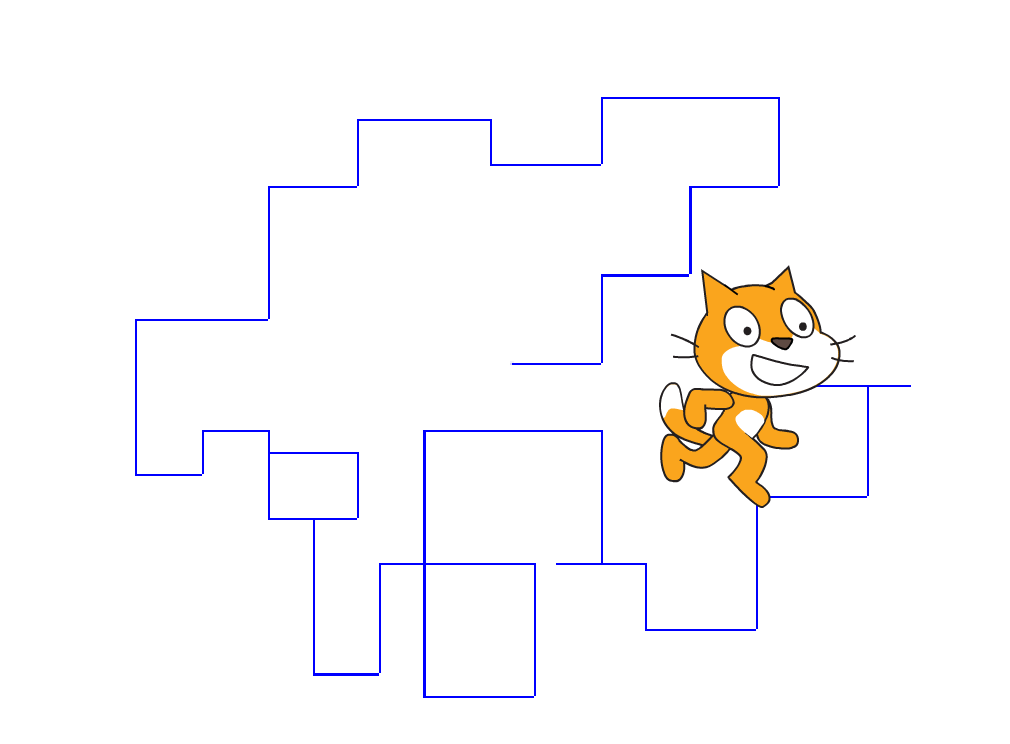
\includegraphics[scale=\scaleecran]{ecran-05-ex1} 
\end{center}



\textbf{Blocs utiles.}
\begin{center}
  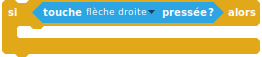
\includegraphics[scale=\scalebloc]{bloc-05-ex1}
\end{center}

\end{activite}



\begin{activite}

Maintenant Scratch doit tracer un triangle en suivant les indications de l'utilisateur.

\begin{center}
  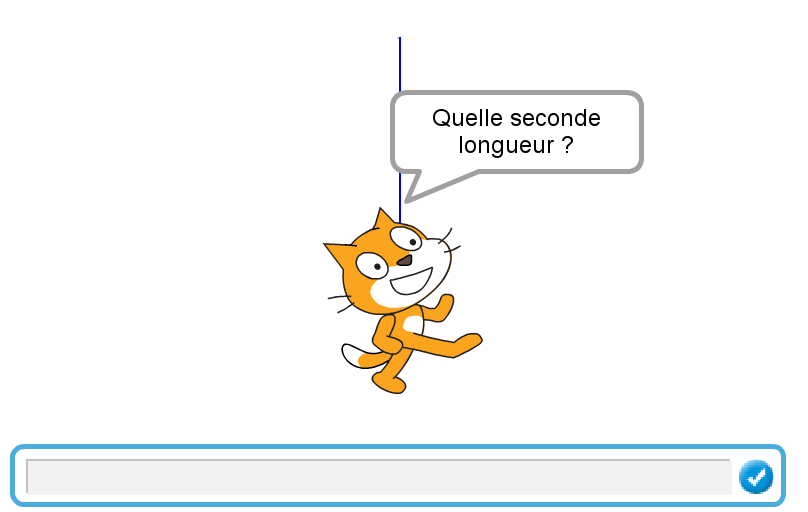
\includegraphics[scale=\scaleecran]{ecran-05-ex2} 
\end{center}


\myfigure{0.9}{
\footnotesize  \tikzinput{figure-05-ex2}
} 


\begin{itemize}
  \item \'Etape 0. Scratch part du point $(0,100)$ et est orienté vers le Sud ($180$\textdegree).
  
  \item \'Etape 1. Demander à l'utilisateur la longueur du premier côté, puis faire avancer Scratch vers le bas du nombre de pas de la réponse.
  
  \item \'Etape 2. Demander à l'utilisateur un angle, puis orienter Scratch selon la valeur répondue.
   
  \item \'Etape 3. Demander à l'utilisateur la longueur du deuxième côté et faire avancer Scratch.
  
  \item \'Etape 4. Scratch retourne au point de départ $(0,100)$.
\end{itemize}

\bigskip

\textbf{Blocs utiles.}
Il est possible de poser une question, d'attendre la réponse, et d'utiliser la valeur répondue à l'aide de la variable \og réponse \fg{}.

\begin{center}
  
\includegraphics[scale=\scalebloc]{bloc-05-ex2a}
  \qquad\qquad\qquad
  
\includegraphics[scale=\scalebloc]{bloc-05-ex2b}
\end{center}

\end{activite}



\begin{activite}
\sauteligne

\begin{enumerate}
  \item Dans un premier temps, Scratch demande le prénom de l'utilisateur et répond \og Bonjour ...\fg{} avec le prénom donné.
  
  \item Dans un second temps, Scratch demande l'âge de l'utilisateur et trace un polygone avec autant de côtés que cet âge.
  
  Par exemple si l'âge est $11$, alors Scratch exécute $11$ fois : avancer de $50$, puis tourner de $360/11$.

\end{enumerate}
\begin{center}
  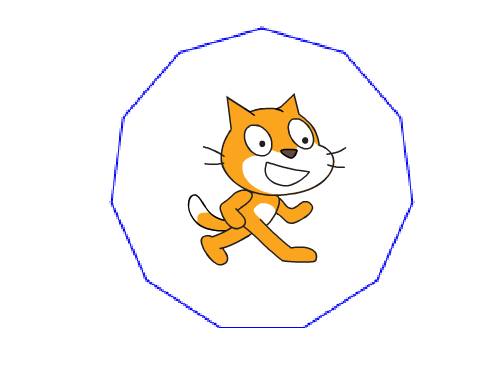
\includegraphics[scale=\scaleecran]{ecran-05-ex3} 
\end{center}



\textbf{Blocs utiles.} Voici deux façons de faire dire à Scratch deux mots. Soit l'un après l'autre, soit en regroupant les deux mots en une seule phrase.
\begin{center}
  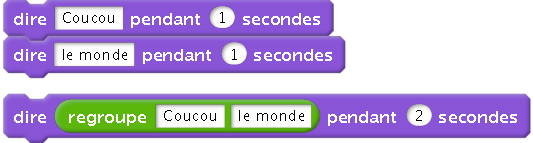
\includegraphics[scale=\scalebloc]{bloc-05-ex3}
\end{center}

\end{activite}


\ifx \displaysolutions \myzero
\else
\begin{code}
\onesolution{Entrée/Sortie}{Activité 1}{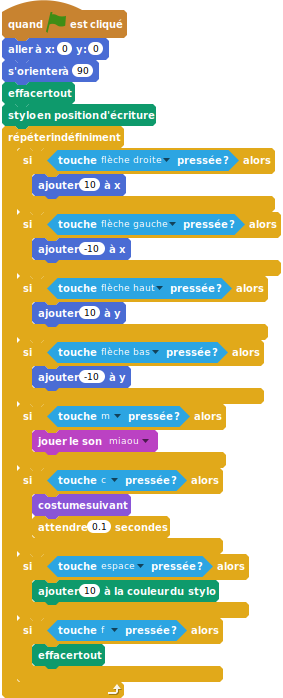
\includegraphics[scale=\scalesolution]{code-05-ex1}}
\onesolution{Entrée/Sortie}{Activité 2}{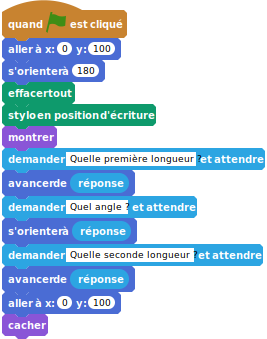
\includegraphics[scale=\scalesolution]{code-05-ex2}}
\onesolution{Entrée/Sortie}{Activité 3}{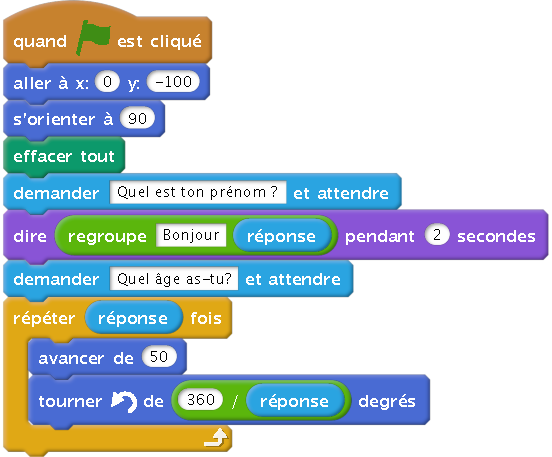
\includegraphics[scale=\scalesolution]{code-05-ex3}}    
\end{code}
\fi


\end{document}

